\documentclass[../main.tex]{subfiles}

\begin{document}

OpenSGX~\cite{opensgx} is a platform that provides a
software emulation layer enabling the execution of SGX instructions
\textit{without} the possession of SGX hardware. Specifically, OpenSGX
implements a hardware emulation layer, implementing SGX's instructions
and data structure as per \Intel's specification \footnotemark, and an
OS emulation layer, providing access to wrapper functions for
privileged SGX instructions (instructions, such as EADD and EINIT,
used to bootstrap an enclave fall under this category)\footnotemark.

Programs that run on top of OpenSGX consist of the trusted code and a
wrapper program which initializes the enclave and provides the trusted
code with an interface to \texttt{sgx-lib}, a library that contains
wrapper functions for user-level SGX instructions.

\Intel's SGX specification does not detail how an enclave program may
invoke system calls\footnotemark; OpenSGX specifies an interface which
allows an enclave program to invoke \texttt{libc} functions. The
interface works as follows:

\begin{enumerate}
  \item The enclave program writes the arguments for the system call
    into a shared area of memory called a \textit{stub}
  \item The enclave program invokes EEXIT, exiting enclave mode, and
    executes a pre-defined handler called a \textit{trampoline} which
    invokes the system call
  \item After the system call is complete, results are written to into
    the \textit{stub} and ERESUME is called, resuming the execution of the
    enclave program
\end{enumerate} By creating this interface, writing code for OpenSGX
is akin to writing C code, making the development process
familiar. Figure~\ref{fig:opensgxdes} illustrates the high level
design of OpenSGX.

\begin{figure}[H]
  \centering
  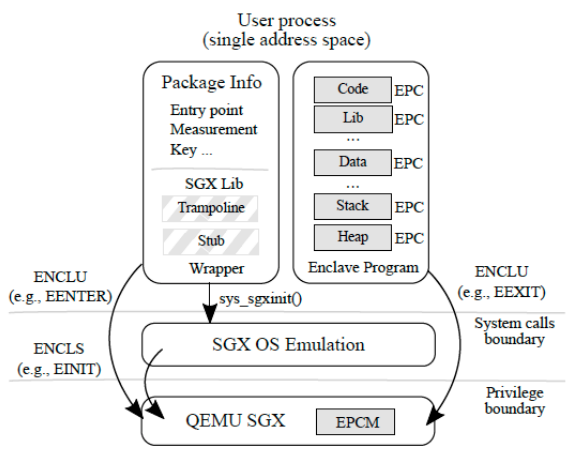
\includegraphics[scale=0.4]{images/opensgx-design.png}
  \caption{High level design of OpenSGX. Grey boxes indicate protected
    areas of memory. Striped boxes indicate shared areas.}
  \label{fig:opensgxdes}
\end{figure}

OpenSGX also provides a tool-chain for automating tasks such as
compiling and signing binaries, generating signing keys, and verifying
and executing correctly signed binaries. However, it is imperative to
note that OpenSGX does not provide the same security guarantees as
SGX; it does not encrypt the enclave memory region, for example. Yet,
it has proven to be useful as a platform for testing the design of our
system, and measuring its performance.

\addtocounter{footnote}{-3}

\stepcounter{footnote}\footnotetext{A few SGX instructions are not
  implemented by OpenSGX including: Debugger Read(EDBGRD) and Debugger
  Write (EDBGWR) which are used to debug an SGX program. However,
  OpenSGX includes a GDB plug-in that performs the same
  task. Furthermore, some instructions are not implemented as they
  were not deemed necessary such as EREMOVE. EREMOVE is called to
  reclaim memory after an SGX program terminates, but it is not
  necessary as only one enclave can run at a time on top of a single
  OpenSGX instance.}

\stepcounter{footnote}\footnotetext{The OS emulation layer's
  implementation was not guided by \Intel's SGX specification, a
  consequence of \Intel not specifying the interface for invoking
  privileged SGX instructions}

\stepcounter{footnote}\footnotetext{Simply put, the enclave program
  cannot invoke I/O system calls directly as any code executed by the
  enclave program must be part of the signed binary. System calls for
  I/O operations, however, delegate work to driver software which
  changes from machine to machine based on the hardware
  provider. Consequentially, allowing arbitrary system calls from
  within the enclave creates a large attack surface.}

\end{document}
